% !TeX root = trigonometric-functions.tex

\chapter{Analysis of Trigonometric Functions}

In this section we examine the derivative, the rate of change, of the trigonometric functions.
There are two approaches: geometric and algebraic.
In both cases, the central concept is that the smaller the length of an arc, the closer the ratio of the arc to the chord with the same endpoints is to one.

\section{The ratio of the length of an arc to its chord}

Figure~\ref{fig.arcs-and-chords} shows four arcs and the chords with the same endpoints. The arcs subtend central angles of $80^\circ, 60^\circ, 40^\circ, 5^\circ$.

The Figure is problematic. As the arcs get smaller, the difference between the length of the arc and the length of the chord is very small. Of course this is what we want but it is difficult to give an estimate of this difference.

\begin{figure}[hbt]
\begin{center}
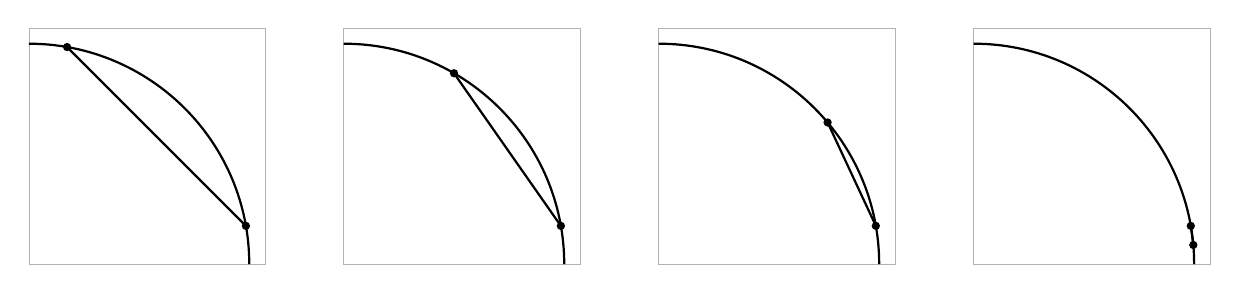
\begin{tikzpicture}
\draw[very thin,white!70!black] (0,0) rectangle +(3,3);
\draw[thick] (2.8,0) arc[start angle=0,end angle=90,radius=2.8cm];
\coordinate (s1) at (10:2.8);
\fill (s1) circle (1.5pt);
\coordinate (t1) at (80:2.8);
\fill (t1) circle (1.5pt);
\draw[thick] (s1) -- (t1);
\begin{scope}[xshift=4cm]
\draw[very thin,white!70!black] (0,0) rectangle +(3,3);
\draw[thick] (2.8,0) arc[start angle=0,end angle=90,radius=2.8cm];
\coordinate (s2) at (10:2.8);
\fill (s2) circle (1.5pt);
\coordinate (t2) at (60:2.8);
\fill (t2) circle (1.5pt);
\draw[thick] (s2) -- (t2);
\end{scope}
\begin{scope}[xshift=8cm]
\draw[very thin,white!70!black] (0,0) rectangle +(3,3);
\draw[thick] (2.8,0) arc[start angle=0,end angle=90,radius=2.8cm];
\coordinate (s3) at (10:2.8);
\fill (s3) circle (1.5pt);
\coordinate (t3) at (40:2.8);
\fill (t3) circle (1.5pt);
\draw[thick] (s3) -- (t3);
\end{scope}
%\begin{scope}[xshift=12cm]
%\draw[very thin,white!70!black] (0,0) rectangle +(3,3);
%\draw[thick] (2.8,0) arc[start angle=0,end angle=90,radius=2.8cm];
%\coordinate (s4) at (10:2.8);
%\fill (s4) circle (1.5pt);
%\coordinate (t4) at (20:2.8);
%\fill (t4) circle (1.5pt);
%\draw[thick] (s4) -- (t4);
%\end{scope}
\begin{scope}[xshift=12cm]
\draw[very thin,white!70!black] (0,0) rectangle +(3,3);
\draw[thick] (2.8,0) arc[start angle=0,end angle=90,radius=2.8cm];
\coordinate (s4) at (5:2.8);
\fill (s4) circle (1.5pt);
\coordinate (t4) at (10:2.8);
\fill (t4) circle (1.5pt);
\draw[thick] (s4) -- (t4);
\end{scope}
\end{tikzpicture}
\caption{Arcs and the corresponding chords}\label{fig.arcs-and-chords}
\end{center}
\end{figure}
Alternatively, consider regular polygons inscribed within a circle (Figure~\ref{fig.regular-polygons}.
The more sides in the polygon, the closer its perimeter is to the circumference of the circle.
The circumference of the circle divided by the number of sides is the length of arcs with the same endpoints as the sides.
Since the ratio of the circumference of the circle to the perimeter of an inscribed polygon approaches 1 as the number of sides increases, so does the ratio of the length of an arc to a chord (see \geoproject{g.polygon}).

\begin{figure}[hbt]
\begin{center}
\begin{tikzpicture}
\draw[very thin,white!70!black] (-2,-2) rectangle +(4,4);
\coordinate (o1) at (0,0);
\coordinate (a1) at (1.8,0);
\node[draw, name path = circle] at (o1)
    [circle through = (a1)] {};
\foreach \node/\angle in {a2/120,a3/240} {
  \coordinate (\node) at (\angle:1.8);
}
\draw[thick,blue] (a1) -- (a2) -- (a3) -- cycle;
\begin{scope}[xshift=5.5cm]
\draw[very thin,white!70!black] (-2,-2) rectangle +(4,4);
\coordinate (o2) at (0,0);
\coordinate (b1) at (1.8,0);
\node[draw, name path = circle] at (o2)
    [circle through = (b1)] {};
\foreach \node/\angle in
  {b2/45,b3/90,b4/135,b5/180,b6/-135,b7/-90,b8/-45} {
  \coordinate (\node) at (\angle:1.8);
}
\draw[thick,blue] (b1) -- (b2) -- (b3) -- (b4) -- (b5) -- (b6) -- (b7) -- (b8) -- cycle;
\end{scope}
\begin{scope}[xshift=11cm]
\draw[very thin,white!70!black] (-2,-2) rectangle +(4,4);
\coordinate (o3) at (0,0);
\coordinate (c1) at (1.8,0);
\node[draw, name path = circle] at (o3)
    [circle through = (c1)] {};
\foreach \node/\angle in
  {c2/22.5,c3/45,c4/67.5,c5/90,c6/112.5,c7/135,
   c8/157.5,c9/180,c16/-22.5,c15/-45,c14/-67.5,
   c13/-90,c12/-112.5,c11/-135,c10/-157.5} {
  \coordinate (\node) at (\angle:1.8);
}
\draw[thick,blue] (c1) -- (c2) -- (c3) -- (c4) -- (c5) -- (c6) --
  (c7) -- (c8) -- (c9) -- (c10) -- (c11) -- (c12) -- (c13) --
  (c14) -- (c15) -- (c16) -- cycle;
\end{scope}
\end{tikzpicture}
%\includegraphics[width=\textwidth,keepaspectratio]{figure21}
\caption{Regular polygons inscribed within a circle}\label{fig.regular-polygons}
\end{center}
\end{figure}

To check this numerically, let us compute the lengths of the arcs, the lengths of the chords and their ratio.
The length of an arc subtending an angle of $\theta$ degrees is $2\pi\disfrac{\theta}{360}$.
By the law of cosines the length of a chord $c$ subtending is:
\[
c^2=a^2+b^2-2ab\cos\theta\,.
\]
in the unit circle $a=b=1$ so:
\[
c=\sqrt{2-2\cos\theta)}\,.
\]
For the arcs and chords in Figure~\ref{fig.arcs-and-chords} we have:
\[
\begin{array}{|r|r|r|r|}
\hline
\multicolumn{1}{|c}{\textrm{Angle}} &
\multicolumn{1}{|c}{\textrm{Arc length}} &
\multicolumn{1}{|c}{\textrm{Chord length}} &
\multicolumn{1}{|c|}{\textrm{Ratio}}\\\hline
80 & 1.396 & 1.286  & 1.090\\\hline
60 & 1.047 & 1.000  & 1.047\\\hline
40 & 0.698 & 0.684 & 1.006\\\hline
5  & 0.087 & 0.087 &1.000 \\\hline
\end{array}
\]

%\begin{figure}[H]
\begin{wrapfigure}[12]{r}{.5\textwidth}
\begin{center}
\vspace{-3ex}
\begin{tikzpicture}[scale=1.3]
  \draw[thin] (-2.2,0) -- (2.2,0);
  \draw[thin] (0,-2.2) -- (0,2.2);
  \coordinate[label = above left:$A$]  (A) at (-2,0);
  \coordinate[label = above right:$B$] (B) at (2,0);
  \coordinate[label = above left:$O$] (O) at (0,0);
  \fill (A) circle (1pt);
  \fill (B) circle (1pt);
  \fill (O) circle (1pt) node[above right,xshift=11pt] {$x$} 
    node[below right,xshift=11pt] {$x$};
  \coordinate (P) at (40:2);
  \fill[red] (P) circle (1.5pt) node[above right] {$P$};
  \coordinate (Q) at (-40:2);
  \node[draw, name path = circle] at (O)
    [circle through = (A)] {};
  \draw[red,very thick] (B)
    arc[start angle=0,end angle=40,radius=2cm];
  \draw[red,very thick] (B)
    arc[start angle=0,end angle=-40,radius=2cm];
  \node[red] at (2.1,.8) {$x$};
  \node[red] at (2.1,-.8) {$x$};
  \draw[very thick,blue] (P) -- node[below left] {$\sin x$}
    (P |- O) coordinate (D);
  \draw[very thick,blue] (D) -- node[above left] {$\sin x$} (Q);
  \fill (D) circle (1pt) node[below right] {$D$};
  \fill[blue] (P) circle (1pt) node[above right] {$P$};
  \fill[blue] (Q) circle (1pt) node[below right] {$Q$};
  \draw (Q) -- (O) -- (P);
\end{tikzpicture}
%\includegraphics[width=.5\textwidth,keepaspectratio]{figure22}
\caption{Ratio of $\sin x$ to $x$}\label{fig.ratio-of-sine-to-x}
\end{center}
%\end{figure}
\end{wrapfigure}

Let us now compute:
\[
\lim_{x \rightarrow 0} \disfrac{\sin x}{x} = \lim_{x \rightarrow 0} \disfrac{2\sin x}{2x}\,.
\]
From Figure~\ref{fig.ratio-of-sine-to-x}) we see that this is the ratio the length of the chord $PQ$ to the length of the arc $PQ$.
But we have shown that this ratio converges to $1$ as the subtended angle tends to $0$. Therefore:
\[
\lim_{x \rightarrow 0} \disfrac{\sin x}{x} = 1\,.
\]

\bigskip\bigskip\bigskip

\section{The geometric approach}
In this approach, the limit $\lim_{x \rightarrow 0} \disfrac{\sin (x+h)-\sin x}{h}$ is computed by looking at the geometric meaning of each component of the expression.
In Figure~\ref{fig.geometric-computation} $x$ is the length of the arc $B$ to point $P_x$, $h$ is the length of the arc from $P_x$ to $P_{x+h}$, and $x+h$ is the sum of the two arc lengths from $B$ to $P_{x+h}$.
Note that the length of an arc in the unit circle is the same as the central angle (in radians) that it subtends.

\begin{figure}[hbt]
\begin{center}
\begin{tikzpicture}[scale=.9]
\coordinate (O) at (0,0);
\coordinate (A) at (0,10);
\coordinate (B) at (10,0);
\fill (O) circle (2pt)
  node[below left] {$O$}
  node[right,xshift=18pt,yshift=6pt] {$x$}
  node[above right,xshift=10pt,yshift=12pt] {$h$};
\fill (A) circle (2pt) node[left] {$A$};
\fill (B) circle (2pt) node[below] {$B$};

\draw[very thick,name path=axes] (B) -- (O) -- (A);
\draw[very thick,name path=arc] (10,0)
  arc[start angle=0, end angle=90, radius=10]
  node[very near start,right] {$x$}
  node[midway,right,yshift=4pt] {$h$};
\draw[very thick,red] (10,0)
  arc[start angle=0, end angle=30, radius=10];
\draw[very thick,blue] (30:10)
  arc[start angle=30, end angle=70, radius=10];

\path[name path=px] (O) -- (30:11);
\path [name intersections={of=arc and px,by={Px}}];
\fill (Px) circle (2pt) node[above right] {$P_x$};

\draw[very thick,name path=pxd] (Px) -- (Px |- O);
\path[name intersections={of=pxd and axes,by={D}}];
\fill (D) circle (2pt) node[below] {$D$};

\path[name path=pxh] (O) -- (70:11);
\path [name intersections={of=arc and pxh,by={Pxh}}];
\fill (Pxh) circle (2pt)
  node[above right] {$P_{x+h}$}
  node[below right,yshift=-10pt] {$\theta$};

\draw[very thick,name path=pxh] (Pxh) -- (Pxh |- O);
\path [name intersections={of=pxh and axes,by={H}}];
\fill (H) circle (2pt) node[below] {$H$};

\draw[very thick,dashed,name path=pxpxh] (Px) -| (Pxh);
\path [name intersections={of=pxh and pxpxh,by={G}}];
\fill (G) circle (2pt) node[left] {$G$};

\draw (D) rectangle +(10pt,10pt);
\draw (G) rectangle +(10pt,10pt);
\draw (H) rectangle +(10pt,10pt);

\draw[very thick,dotted] (O) -- (Pxh);
\draw[very thick,dotted] (O) -- (Px);
\draw[very thick,dashed] (Pxh) -- (Px);

\path (D) -- node[left] {$\sin x$} (Px);
\path (H) -- node[left] {$\sin x$} (G);
\path (G) -- node[left] {$\sin(x+h)\!-\!\sin x$} (Pxh);
\end{tikzpicture}
\caption{Geometric computation of the limit}\label{fig.geometric-computation}
\end{center}
\end{figure}

$P_xD$ and $P_{x+h}H$ are perpendicular to the $x$-axis and $P_xG$ is perpendicular to $P_{x+h}H$.
We are interested in the angle $\theta$, which is the difference between two angles:
\[
\theta=\angle GP_{x+h}P_x= \angle OP_{x+h}P_x - \angle OP_{x+h}H\,.
\]
Since all radii are equal, $\triangle OP_{x+h}P_x$ is isoceles, and since the sum of the angles of a triangle is $\pi$ we have:
\[
\angle OP_{x+h}P_x=\frac{1}{2}(\pi - h)\,.
\]
From the sum of the angles in the right triangle $\triangle OP_{x+h}H$ we have:
\[
\angle OP_{x+h}H = \left(\pi-\frac{\pi}{2}-(x+h)\right) = \left(\frac{\pi}{2}-(x+h)\right)\,.
\]
Therefore:
\[
\theta = \angle GP_{x+h}P_x=\frac{1}{2}(\pi - h) - \left(\frac{\pi}{2}-(x+h)\right) = x+\frac{h}{2}\,.
\]
In the right triangle $\triangle P_xGP_{x+h}$:
\[
\cos \theta = \frac{\sin(x+h)\!-\!\sin x}{P_{x+h}P_x}\approx \frac{\sin(x+h)\!-\!\sin x}{h}\,,
\]
taking the length of the arc $h$ as an approximation of the chord $P_xP_{x+h}$. Taking the limit:
\[
\sin' x = \lim_{h\rightarrow 0} \frac{\sin(x+h)\!-\!\sin x}{h} =  \lim_{h\rightarrow 0}\cos \theta = \lim_{h\rightarrow 0} \cos \left(x+\frac{h}{2}\right) = \cos x\,.
\]

\section{The algebraic approach}

This approach is shorter and also relies on the limit $\lim_{x\rightarrow 0} \disfrac{\sin x}{x} = 1$. We use the identity:
\[
\sin(\alpha) -\sin\beta = 2\sin \frac{\alpha-\beta}{2}\cos \frac{\alpha+\beta}{2}\,,
\]
and the continuity of both the sine and cosine functions:
\begin{eqnarray*}
\lim_{h\rightarrow 0} \frac{\sin(x+h)\!-\!\sin x}{h}&=& \lim_{h\rightarrow 0} \frac{2\sin(\frac{h}{2})\cos(x+\frac{h}{2})}{h}\\
&=&\lim_{h\rightarrow 0}
  \left[
    \left( 
      \frac{\sin(\frac{h}{2})}{\frac{h}{2}}
    \right)
    \cos\left( x+\frac{h}{2} \right)
   \right]\\
& =& \cos x\,.
\end{eqnarray*}
Students can be asked to justify each of the steps in this computation.

The choice between the two approaches depends on the which skills we wish to reinforce in the students.
Clearly, the geometric approach requires the ability to follow a non-trivial geometric derivation. 
The algebraic approach depends on understanding the concepts of continuity and limits.

We emphasize that both approaches are based on:
\[
\lim_{h\rightarrow 0} \frac{\sin(x+h)\!-\!\sin x}{h} =1\,,
\]
that was proved at the beginning of this chapter.

We refer the reader to the article by Josevich \cite{josevich} who shows how the derivative can be obtained from the principles of classical mechanics.
